\documentclass[8pt, a4paper]{extarticle}
\usepackage{scrextend}
\changefontsizes{6.5pt}
\usepackage[a4paper, top=0.02in, bottom=0.02in, left=0.02in, right=0.02in, heightrounded]{geometry} % Minimal margins
\usepackage{amsmath,amssymb,amsthm}
\usepackage{booktabs}         % Professional table spacing
\usepackage{parskip}          % Clean paragraph
\usepackage{enumitem}
\usepackage{graphicx} % Required for \includegraphics
\usepackage{ragged2e}
\usepackage{microtype}
\usepackage{fourier}
\usepackage[absolute,overlay]{textpos}
\usepackage{array} % For better column definitions
\usepackage{booktabs} % For improved table aesthetics
\usepackage{subfiles}                % For subfiles compilation
%%%%%%%%%%%%%%%%%%% C CODE STYLING %%%%%%%%%%%%%%%%%%%%%%%%%%%%%
\usepackage{xcolor}
\usepackage{listings}
\usepackage{soul}
\color{black!92}
\setlength{\parindent}{0pt}
% Define custom colors for C syntax highlighting
\definecolor{CKeyWord}{rgb}{0.8,0.1,0.1}      % For C keywords (e.g., int, return)
\definecolor{CBackground}{rgb}{0.95,0.95,0.95} % Background color for code blocks
\definecolor{CComment}{rgb}{0.0,0.5,0.0}        % Comment color
\definecolor{CString}{rgb}{0.1,0.1,0.8}         % String literal color
\definecolor{CRule}{rgb}{0.5,0.5,0.5}           % Frame rule color
\definecolor{CNumber}{rgb}{0.6,0.6,0.6}         % Line number color

% Define a custom listing style for C code
\lstdefinestyle{CStyle}{
	language=C,
	basicstyle=\footnotesize\ttfamily,
	backgroundcolor=\color{CBackground},
	commentstyle=\color{CComment},
	keywordstyle=\color{CKeyWord}\bfseries,
	stringstyle=\color{CString},
	numbers=false,
	numberstyle=\tiny\color{CNumber},
	stepnumber=1,
	numbersep=10pt,
	showspaces=false,
	showstringspaces=false,
	breaklines=true,
	frame=single,
	rulecolor=\color{CRule},
	tabsize=1,
	captionpos=b,
	columns=fullflexible,
	keepspaces=false,
	aboveskip=3pt,           % Reduce space above
	belowskip=3pt,           % Reduce space below
	xleftmargin=4pt,        % Increase left margin
	xrightmargin=4pt,       % Increase right margin
}

% Define a new environment for C code blocks using the custom style.
% Optional arguments can be passed to adjust settings further.
\lstnewenvironment{cc}[1][]{
	\lstset{style=CStyle, autogobble=true, #1}
}{}
%
\usepackage{minted}
\raggedbottom
\setlist[itemize]{leftmargin=1em}
\newcommand{\dist}[2]{\left\langle #1,\, #2 \right\rangle}
\setlength{\TPHorizModule}{0.1mm} % Set horizontal units to millimeters
\setlength{\TPVertModule}{0.1mm}  % Set vertical units to millimeters
\usepackage{multicol}
\setlength{\parindent}{0pt}
\setlength{\parskip}{5pt plus 1pt minus 1pt}
\usepackage{setspace}
\setstretch{0.98}
\pagestyle{empty}
\setlength{\parskip}{0pt}      % space between paragraphs
\setlength{\parindent}{0pt}    % optional: remove indentation
\setlist{nosep, topsep=0pt, partopsep=0pt, parsep=0pt, itemsep=0pt}
% Redefine the textblock environment
\let\originaltextblock\textblock
\let\endoriginaltextblock\endtextblock
% Adjust vertical centering of the existing \warning symbol
\let\oldwarning\warning
\renewcommand{\warning}{\raisebox{0.3ex}{\oldwarning}}

\makeatletter
\renewcommand{\hline}{\noalign{\vskip 2px}\hrule\@height\arrayrulewidth\@width\linewidth\noalign{\vskip 2px}}
\makeatother

\renewenvironment{textblock}[2][]{%
	\originaltextblock[#1]{#2}%
	\fcolorbox{red}{white}{%
		\begin{minipage}{#2}%
			}{%
		\end{minipage}%
	}%
	\endoriginaltextblock
}


\begin{document}
\begin{titlepage}
	\centering
	% Moderately larger size hierarchy
	\makeatletter
	\renewcommand{\Huge}{\@setfontsize\Huge{26pt}{30pt}}
	\renewcommand{\LARGE}{\@setfontsize\LARGE{20pt}{24pt}}
	\renewcommand{\Large}{\@setfontsize\Large{16pt}{20pt}}
	\renewcommand{\large}{\@setfontsize\large{13pt}{16pt}}
	\makeatother

	\vspace*{1cm}
	{\Huge \textbf{Responsible Software - CheatSheet}} \\
	\vspace{20pt}
	{\LARGE IN~BA5 - Cécile Hardebolle
	} \\
	\vspace*{1cm}
	{\Large Notes by Ali EL AZDI} \\
	\vfill

	{\large January 16th, 2026}
	\vspace*{60px}
\end{titlepage}

\noindent
\\
\newpage
\\
\noindent\begin{minipage}[t]{0.48\textwidth}
	\fbox{
		\begin{minipage}[t]{1\textwidth}
			\underline{\textbf{INTRO.}}
			\textbf{Responsible Software.} Software engineered in a responsible\textit{(ethical)} way.\\
			1. With a goal to do good. 2. While preventing avoidable negative impacts.\\
			3. Taking people, other systems, social structures and our planet into account.\\
			\textbf{Active Responsibility.} anticipating/preventing negative impacts before occurring.\\
			\textbf{Ethics.} Principles/standards that guide human behavior in various contexts.\\
			\textit{Metaethics.} "what does it mean for an action to be right ?"\\
			\textit{Normative.} "how should people act in general (moral principles)?"\\
			\textit{Applied. (Our approach)} "how can i act ethically in a real-world situation?"
			\hline
			\begin{minipage}[t]{0.41\textwidth}
				\textbf{Technical decisions} can have \textit{ethical} implications.\\
				\textbf{Ethical Issue.} any situation that may compromise respect of ethical value/principle.\\
				\textbf{Ethical Agency.} capacity to take actions that align with ethical values and principles.\\
				\textbf{Ethical Sensitivty.} ability to\\
				- recognize ethical issues (awareness)\\
				- identify their impact: who, what
			\end{minipage}\hfill
			\begin{minipage}[t]{0.59\textwidth}
				\textbf{Ethical Decision Making.}\\
				1. \textbf{Recognize}(knowledge+experience+habits)\\
				2. \textbf{Evaluate}(cognitive+reason+affective) \;
				3. \textbf{Act}.\\
				\textbf{Ethical Lenses.}\\
				1. \textbf{Desirability.} product corresponds to what people want.\\
				2. \textbf{Viability.} product generates profits for a business.\\
				3. \textbf{Feasibility.} product can be created with existing or new technology.\\
				\textbf{Fourth criterion (Isaac et al.).} add \textbf{Ethicality.}
			\end{minipage}
			\hline
			\textbf{Ethical Dilemmas.} decision between multiple alternatives, all conflict with ethical values/principles.
			\textit{None of the options override the other, wrong-wrong choice.}\\
			\begin{minipage}[t]{0.33\textwidth}
				\textbf{Moral side.}\\
				Emotions should be used explicitely/intentionally for \ul{responsible} design (Roeser). In response to moral issues or motivating immoral behavior.
			\end{minipage}\hfill\vline\hfill
			\begin{minipage}[t]{0.66\textwidth}
				\textbf{Cognitive side (Normative Ethics).}\\
				- \textbf{Utilitarianism(Consequences).} choose the greatest good for greatest number\\
				- \textbf{Deontology(Action).} do right according to universal principles\\
				- \textbf{Virtue(Person).} act as a virtuous person\\
				- \textbf{Care(Relationships).} mutual responsibility/care for each other
			\end{minipage}\\
			\textit{Trolley problem.} thought experiment, \textbf{choice}: do nothing $\to$ runaway trolley kill people,
			\ul{or} intervening $\to$ fewer people die. tests which moral principles justify action vs. inaction.\\
			\begin{minipage}[t]{0.33\textwidth}
				\textbf{Ethical Decision Frameworks.}\\
				1. Identify the ethical issues\\
				2. Get the facts\\
				3. Evaluate alternative actions with \textit{several ethical theories}\\
				4. Choose an option and "test" it\\
				5. Implement your decision and \\reflect on the outcome.
			\end{minipage}\hfill\vline\hfill
			\begin{minipage}[t]{0.66\textwidth}
				\textbf{Example questions for brainstorming}\\
				- Who will use your product on a daily basis?\\
				- Who is in geographical proximity with the users of your product?\\
				- Who is in social proximity with the users of your product?\\
				- Who is involved in the maintenance of your product?\\
				- Who provides services that are needed to run your product?\\
				- Who provides funding?\\
				- Which communities are active in the application domain?
			\end{minipage}
			\hline
			\textbf{Stakeholder} Individuals/groups/organizations/institutions/societies that might reasonably be affected by technology.
			\textbf{Direct Stakeholder.} \textit{in contact} with the product\\
			\textbf{Indirect Stakeholder.} affected through \textit{consequences of the usage} of the software\\
			\begin{minipage}[htp]{0.74\textwidth}
				\ul{\textbf{Stakeholder analysis.}} Identifying every entity that can be affected by software positively/negatively.
				1. Find all stakeholders possible using questions.\\
				2. Use Direct vs Indirect Chart to find new stakeholders.\\
				Additional Methodologies: \textit{Ethix. add unintended stakeholders}, \textit{Mitchell. add attributes to stakeholders}, \textit{SAS. use different chart with scale for impact from product and influence on the product}.
			\end{minipage}\hfill
			\begin{minipage}[htp]{0.25\textwidth}
				\centering\vspace*{-10px}
				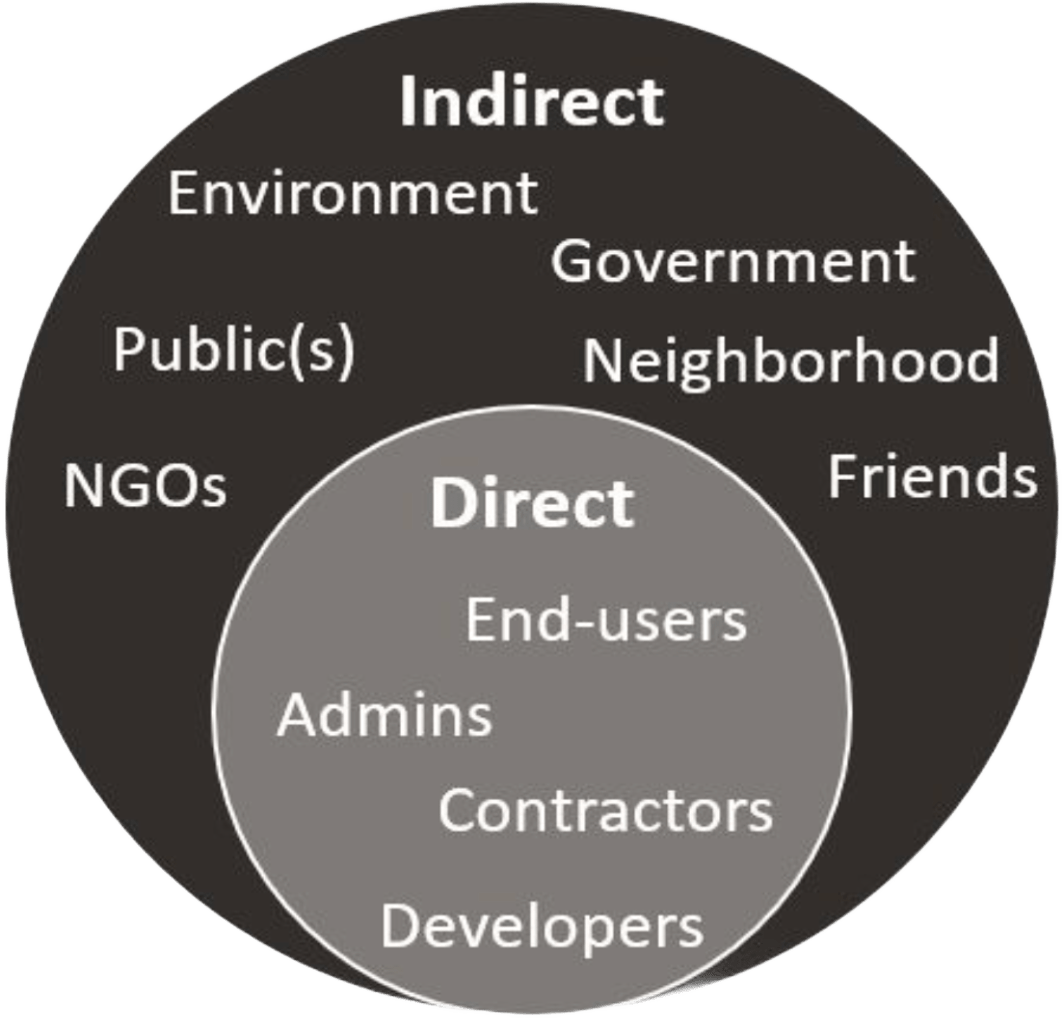
\includegraphics[width=0.75\textwidth]{direct-indirect.png}
			\end{minipage}\hline
			\ul{\textbf{Ethical Speculation.}} How to think, not what to think - anticipate potential impacts on stakeholders.\\
			Create a fictional story in two parts. (\textit{done at the early design phase})\\
			\begin{minipage}[t]{0.44\textwidth}
				\textbf{I. Dark and Pessimistic}\\
				1. Imagine a character that would be negatively impacted by the software\\
				2. Write a pitch that summarizes their story.\\
				3. Find a title.
			\end{minipage}\hfill
			\begin{minipage}[t]{0.54\textwidth}
				\textbf{II. Positive outcome}\\
				1. Identify 1 or 2 main ethical issues represented in your story.\\
				2. Describe the immediate and future consequences.\\
				3. Imagine a happy ending for character.
			\end{minipage}
		\end{minipage}}\\[2px]
	\fbox{\begin{minipage}[t]{1\textwidth}
			\underline{\textbf{SAFETY II.}}
			\small
			\textbf{Levels of analysis.} Macro (societies), Meso (groups/communities), Micro (individuals)\\
			\textbf{Internet Trafic.} 99\% submarine cables: 1.4M km, 4.7B users, 1.2 ZettaBytes (1.2 trillion GB).\\
			\begin{minipage}[htp]{0.49\textwidth}
				\textbf{Internet Benefits (+).} Information access/dissemination, Communication, Social relations/organization, Identity/psychological development, Learning/cognitive development, Production/commerce.
			\end{minipage}\hfill\vline\hfill
			\begin{minipage}[htp]{0.49\textwidth}
				\textbf{Internet Harms (-).} Privacy boundary violations, Social relationship harm, Community damage, Addiction, Cognitive impairment, Information overload, Knowledge/belief distortion, Democratic threats.
			\end{minipage}
			\normalsize
			\textbf{Tension.} Same features enable both benefits/harms $\to$ \textit{social connection enables social harm, information access causes overload, identity spaces blur privacy boundaries}.\\
			\textbf{From micro to macro.}\\
			\textbf{Types of impacts:} lots of individuals, Social structures/institutions, Different for different groups.\\
			\textbf{Areas:} Markets/economy, Knowledge/worldviews, health/well-being, Politics/citizenship, Environment. \textbf{\warning controversy} Complex measurements, causality hard to establish.
			\hline
			\begin{minipage}[t]{0.545\textwidth}
				\textbf{Disinformation.} false info. with intent to deceive.\\
				\textbf{Misinformation.} false info. without intent to deceive\\
				\textbf{Malinformation.} true info. used with harmful intent.\\
				\emph{fake news} $\to$ false information, with or without intent.
			\end{minipage}\hfill\vline\hfill
			\begin{minipage}[t]{0.445\textwidth}
				\textbf{Global risks.} impact on electoral processes \textit{(Brexit, U.S. elections)}, growth of distrust (government/media sources), risks of repression. \textit{socio-technical phenomenon}
			\end{minipage}\\
			\begin{minipage}[htp]{0.44\textwidth}
				\textbf{Cognitive effects.} how we think.\\
				\textbf{Socio-affective effects.} interaction with people and emotions.\\
				\textbf{System 1.} fast/emotional/ activated first as quick response.\\
				\textbf{System 2.} slow/logical/conscious analysis.\\
				\textbf{Illusory truth effect.} repetition increases perceived truthfulness of claims by enhancing familiarity and intuitive/shortcut-based thinking.
			\end{minipage}\hfill\vline\hfill
			\begin{minipage}[htp]{0.55\textwidth}
				\textbf{Socio-affective factors}\\
				- \textbf{Source cues.} perceived credibility (powerful/attractive sources more likely to be believed).\\
				- \textbf{False consensus.} overestimating how many people agree \textit{(climate change denial.\(\sim 6\%)\) in reality, perceived \(\sim 50\%\))}.\\
				- \textbf{Emotions.} strong emotions content/receiver emotional stae increases susceptibility.\\
				- \textbf{Identity resonance.} alignment with personal identity/values increases acceptance.
			\end{minipage}
			\textbf{Continued influence effect}: misinformation continues to influence beliefs even after correction is received and accepted as true.\\
			\textbf{Increased use of digital media shows} greater exposure to misinformation, increased political polarization, decreased trust, and increased hate. \textit{empirical results remain debated and sometimes exaggerated}
			\hline
			\textbf{Publication.} publicly availabling content, \textit{financial}/\textit{political}/\textit{coordinated strategic} incentives.\\
			\textbf{Human publishers.} Influential figures/ordinary users publishing for visibility/revenue, often using \textit{clickbait}/participating in organized campaigns \textit{(coordinated troll operations)}.\\
			\textbf{Social bots.} Automated accounts publishing at scale (\textbf{1--15\%}), they generate \textit{disproportionately large share} of misinformation.\\
			\textbf{Propagation.} content spreading through \textit{reposting}/\textit{liking}/\textit{algorithmic amplification}.\\
			\textbf{Human propagation.} content reshared by real/fake accounts. engagement inflated by paid workers, while moderation reduces resharing \textit{(account bans lowering repost rates)}.\\
			\textbf{Genuine resharing factors.} Resharing driven by \textit{inattention}, \textit{emotional reactions}, and \textit{socio-affective motives} such as signaling group membership or provoking reactions \textit{(outrage)}.\\
			\textbf{Social bots in propagation.} Automated accounts rapidly \textit{repost} and \textit{target influential or opposing users} to maximize visibility and conflict.\\
			\textbf{Recommender systems.} \textit{select, rank, display} content, optimize for \textit{engagement} (\textit{popularity bias}).
			\hline
			\begin{minipage}[t]{0.49\textwidth}
				\ul{\textbf{Ethics Canvas.}} Structure stakeholder, impact, and mitigation info systematically. \\
				\textit{When to use?} Early software development \textit{Brainstorm, visualize, mitigate ethical impacts)}\\
				1. Identify Stakeholders: Who is affected?\\
				2. Ethical Impacts: What are the impacts on them?\\
				3. Actions: How to address these impacts?\hline
				\ul{\textbf{Causal loop diagram.}} to explain complex systems/improve performance/solve issues\\
				focuses on specific issues \textit{(amount of fake news, investment in an auto-detection system)}\\
				Causal links are labeled with a $+$/$-$ longer delays are represented with thicker arrows.
			\end{minipage}
			\begin{minipage}[t]{0.49\textwidth}
				\ul{\textbf{Edge Cases.}} Foresee consequences/identify opportunities for improvement analyzing extreme scenarios.\\
				\textit{When to Use: At all stages,design/major updates/user base growth/audience shifts to address evolving societal impacts.}\\
				– Global Reach: Impact of multicultural/lingual use.\\
				– Mass Adoption: Scalability/infrastructure under high loads.\\
				– Longevity: Long-term use/societal changes/evolving norms
				\hline
				\textbf{System.} collection of organized parts that interact as a whole to reach a state/purpose; modeling simplifies complexity/identify patterns.
			\end{minipage}
		\end{minipage}}\end{minipage}\hspace{8px}
\begin{minipage}[t]{0.49\textwidth}
	\fbox{
		\begin{minipage}[t]{1\textwidth}
			\underline{\textbf{SAFETY I.}}\\
			\textbf{Security.} Prevent the environment from affecting negatively the system. \textit{\warning threat} | \textit{Vulnerability scanning, ethical hacking, security audit, code review}\\
			\textbf{Safety.} Prevent the system from affecting negatively the environment. \textit{\warning hazard} | \textit{Verification and testing, failure modes analysis, Redundancy}\\
			\textbf{Common challenge - human factor} $\to$ consider software as \textbf{socio-technical system}\\
			\textit{Internet, Autonomous vehicles, social media}, human behavior and technical systems constanly influence each other.
			\hline
			\textbf{Malfunction.} software doesn't function/perform normally/as specified.\\
			- Due to unintentional defect/fault/bug$\to$critical consequences(\warning Life/Mission-critical systems)\\
			\textbf{Misuse/Abuse.} attack, diversion, use of software for \textit{nefarious purposes}. \\
			\textbf{Bad/threat actors.} \textit{malicious intent, authorized/unauthorized users}$\to$direct/indirect impact.\\
			\textbf{Unintended use.} use of software in a way not originally intended/not (officially) supported.\\
			$\oplus$ creates opportunities for innovation \textit{use camera to scan documents}
			$\ominus$ \textit{use llm to obtain factual information}\\
			\textbf{Intended use} software used as intended. difficult to anticipate impact due to social \warning scale/time
			\hline
			\textbf{User-Generated Content (UGC).} any content posted by users online \textit{images/videos/texts}\\
			- Published publicly and (usually) not produced by professional/institution \textit{wikipedia}\\
			\warning \textbf{Toxic content.} material harmful/offensive can have negative impact on individuals/communities\\
			\textbf{Types of impacts?} Physical/Financial/Emotional/Relational.\\
			\begin{minipage}[t]{0.47\textwidth}
				\textit{Hate and Harassment.}\\
				Violence threats, Identity misrepresentation\\
				\textit{Self-inflicted harm.} Eating disorder promotion\\
				\textit{Ideological harm.}\\
				Extremism/terrorism, Misinformation\\
				\textit{Exploitation.} Sexual abuse, Scams
			\end{minipage}
			\begin{minipage}[t]{0.53\textwidth}
				\textbf{Central dilemma.} protecting users from toxic content while preserving free speech rights\\
				\textbf{To decide?} \\
				- State (responsible for fulfilling rights), \\
				- Platforms (private actors with business interests), \\
				- People (responsible for the content they publish.
			\end{minipage}\\
			\begin{minipage}[t]{0.5\textwidth}
				\textbf{Hate speech}\\
				- Discriminatory/pejorative of individual/group\\
				- calls out real/perceived "identity factors" of individual/group\\
				- conveyed through any form of \expression (images/memes/\ldots)
			\end{minipage}
			\begin{minipage}[t]{0.5\textwidth}
				\textbf{Free speech.} right to express opinions and to seek, receive, share information/ideas, in any format offline/online, subject to limitations that respect the rights of others and prohibit incitement to discrimination or violence, pillar of democracy.
			\end{minipage}
			\textit{UGC platforms provide channels for hate speech. Easily produced, shared, anonymous, global/diverse audience, realtime, amplified by content recommendation algorithms}\\[-6px]
			\begin{minipage}[htp]{0.001\textwidth}
				\multirow{}{\rotatebox{90}{\textbf{Predicted}}}
			\end{minipage}\hspace*{-8px}
			\begin{minipage}[htp]{0.999\textwidth}
				\begin{minipage}[htp]{0.65\textwidth}
					\begin{tabular}{cc|c|c|}
						\multicolumn{2}{c}{}  & \multicolumn{2}{c}{\textbf{Actual}}                                             \\
						\cline{3-4}
						\multicolumn{2}{c|}{} & Positive                            & Negative                                  \\
						\cline{2-4}
						                      & Positive                            & True Positive (TP)  & False Positive (FP) \\
						\cline{2-4}
						                      & Negative                            & False Negative (FN) & True Negative (TN)  \\
						\cline{2-4}
					\end{tabular}
				\end{minipage}\hfill
				\begin{minipage}[htp]{0.33\textwidth}
					\textbf{Content moderation}:\\
					\textit{False negative}: toxic content that escapes moderation.\\
					\textit{False positive}: wrongful censorship, restricting free speech.
				\end{minipage}
			\end{minipage}\\
			\begin{minipage}[htp]{0.5\textwidth}
				\textbf{TP.}Model predicts positive and is correct\\
				\textbf{Accuracy}                        $= \frac{TP + TN}{TP + TN + FP + FN}  $\\
				\textbf{Positive Predictive Value (PPV)} $= \frac{TP}{TP + FP}                 $\\
				\textbf{Negative Predictive Value (NPV)} $= \frac{TN}{TN + FN}                 $
			\end{minipage}
			\begin{minipage}[htp]{0.5\textwidth}
				\textbf{False Discovery Rate (FDR)}      $= 1 - \text{PPV} = \frac{FP}{TP + FP}$\\
				\textbf{False Omission Rate (FOR)}       $= 1 - \text{NPV} = \frac{FN}{TN + FN}$\\
				\textbf{False Positive Rate (FPR)}       $= \frac{FP}{FP + TN}                 $\\
				\textbf{False Negative Rate (FNR)}       $= \frac{FN}{FN + TP}$
			\end{minipage}
			\hline
			\ul{\textbf{Bad Actors Modelling}} Minimize vulnerabilities via risk assessment and mitigation.\\
			\textit{When to Use: Design phase, prior to updates, audits, incident responses, and improvements.}\\
			\textit{What is a Bad Actor? A person/group exploiting a system for personal goals.}\\
			\begin{minipage}[htp]{0.65\textwidth}
				\textbf{Motivations (might overlap)}:\\
				- Money: Data theft, ransomware, sabotage by competitors.\\
				- Politics: Misinformation/strategic sabotage/infrastructure attacks.\\
				- Entertainment: Attacks on random systems, misinfo. spreading.\\
				- Self-interest: Harassing messages, communication monitoring, location tracking.\\
				- Ideas: Discrediting groups, data leaks, website defacement.
			\end{minipage}
			\begin{minipage}[htp]{0.34\textwidth}
				\textbf{Steps:}
				1. Identify possible malicious users and their motivations.\\
				2. Assess potential consequences for the system and users.\\
				3. Develop measures to prevent these negative outcomes.
			\end{minipage}
			\hline
			\ul{\textbf{Harm Modelling}} anticipate/address potential harms users/stakeholders may encounter.\\
			\textbf{When to Use:} At every stage of project, for every feature, until harm potentials are satisfactory.\\
			\textbf{Evaluate:} 1. The category of use. 2. the types of harms. 3. the magnitude of harm\\
			\small
			\begin{minipage}[t]{0.24\textwidth}
				\textbf{Categories of Use:}\\Harm from\dots\\
				\textit{Intended Use:} correct usage.\\
				\textit{Unintended Use:} unexpected usage.\\
				\textit{Misuse/Abuse:} malicious usage.\\
				\textit{Malfunction:} system failures.
			\end{minipage}\hfill
			\begin{minipage}[t]{0.37\textwidth}
				\textbf{Types of Harm:}\\
				\textit{Humans:} Physical, emotional injury.\\
				\textit{Allocation of Resources:} Opportunity, economic losses.\\
				\textit{Human Rights:} Dignity, liberty, privacy losses; environmental impact.\\
				\textit{Social Systems:} Manipulation, social detriment.
			\end{minipage}\hfill
			\begin{minipage}[t]{0.37\textwidth}
				\textbf{Magnitude of Harm:}\\
				\textit{Severity:} Impact on individual/group well-being.\\
				\textit{Scale:} How broadly the harm affects populations.\\
				\textit{Probability:} Likelihood of harm occurring.\\
				\textit{Frequency:} How often the harm might occur.
			\end{minipage}\normalsize
		\end{minipage}}
	\fbox{
		\begin{minipage}[t]{1\textwidth}
			\underline{\textbf{FAIRNESS I.}} \textbf{Data in Software.} people described by \textbf{attributes} (stored in databases/files), can be \textit{sensitive}.\\
			$\Rightarrow$ \textit{ethical implications} such as \textit{confidentiality, privacy, and fairness}. data is an \textit{imperfect representation of real world}, must be \textit{simplified} to fit context.\\
			\textbf{Data protection law} \textit{(GDPR)} - \textbf{Personal} data: reveals info about \textit{identity}, directly/indirectly. \\
			- \textbf{Special category} data: banned by default. \textit{racial/ethnic origin, pol.\ opinions, rel.\ beliefs, health data.}\\
			\textbf{Nondiscrimination Law} forbids direct/indirect discrimination, when \textbf{apparently} \textit{neutral} practice puts \textit{specific groups} at disadvantage.
			\textit{(Protected Group/Class: Category qualifying for special protection by law/policy)}\\
			\textbf{Proxy Attributes.} Variables that \textbf{correlate} w/ sensitive attributes.\\
			\textbf{Risks \& Outcomes.} can lead to \textbf{indirect discrimination} \textit{(harder to detect)}.\\
			- Software has discriminatory outcomes even in absence of sensitive attributes in data.\\
			\textit{(high school quality)} - correlates w/ income/ethnicity $\rightarrow$ becomes proxy.\\
			\textbf{Fairness.} Equality \textit{opportunities}; operationalized by treating people same. Scope matters: groups not protected law still face ethical harm.\\
			\textbf{Unfairness.} Discrimination, stereotyping, decision errors based irrelevant factors; causing negative impacts via biased software/processes \textit{(women get lower credit limits despite higher income)}.\\
			\textbf{Bias.} Systematic deviation from standard. context-dependent, not always harmful, possible ethical issues.\\
			\textit{affects Problem definition/ideas/solutions/planning; shaped by external factors \textit{(info/org. culture)}}\\
			\begin{minipage}[htp]{0.4\textwidth}
				\vspace*{-10px}
				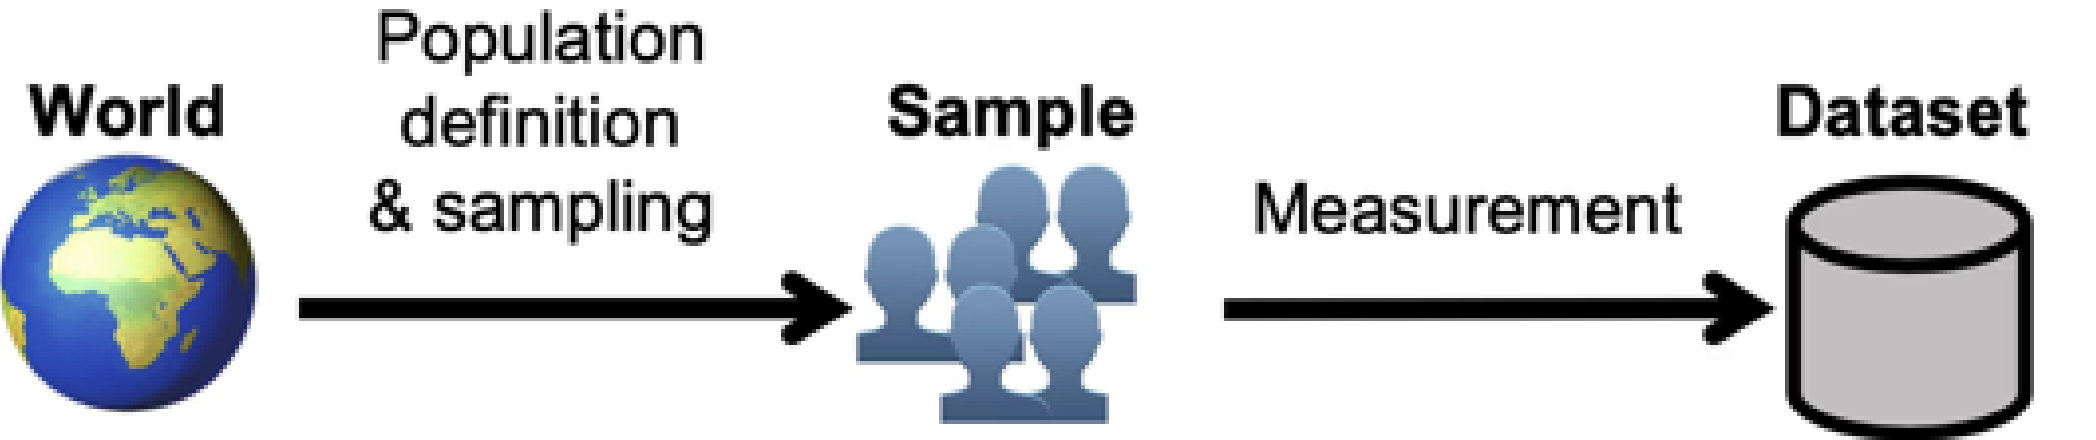
\includegraphics[width=1\textwidth]{data-pipeline.png}
			\end{minipage}
			\begin{minipage}[htp]{0.59\textwidth}
				1. \textbf{Pre-existing bias.} Bias already present world, captured in data \textit{(systemic bias)}.\\
				2. \textbf{Representation bias.} Data inaccurately reflects target population/subgroup \textit{(Sampling: over/under-representation. Population: sampled pop. differs actual users)}.
			\end{minipage}\\
			3. \textbf{Measurement bias.} Methods yield inaccurate values, oversimplify reality, differ accuracy across groups \textit{(blood-oxygen devices more accurate white people vs darker skin due melanin)}.\\
			4. \textbf{Cognitive bias.} Human (often implicit) deviations rational judgment; affects info processing/interpretation; enters via users/designers.\\
			\textbf{Stereotypes.} Generalized beliefs about group \textit{(implicit/explicit; pos/neg/neutral)}; ignore individual differences, reinforced by design assumptions.\\
			\textbf{Group effects.} groups with same opinions/preferences $\to$ reinforce confirmation bias; \textit{(devil's advocate strategy)} doesn't work $\to$ groups with heterogeneous preferences more balanced\\
			$\to$ group-think: phenomena where alternatives are avoided, pseudo-consensus\\
			\textbf{Sunk-cost fallacy.} continuing course of action just due to past investment $\to$ prevents alternatives$\to$product with design flaws
			$\to$ \textbf{Technical debt.} future costs to fix, \textbf{Ethical debt.} ethical consequences/harms\hline
			\ul{\textbf{Inclusive Design.}} design software that benefits the widest range of users by addressing diverse abilities, languages, cultures, and differences.\\
			\begin{minipage}[t]{0.45\textwidth}
				\textit{When to Use: Early in soft. development phases.}\\
				\textbf{1.} Identify needed capabilities for use.\\
				\textbf{2.} Identify and label ”Non-Average Users” (NAUs).\\
				\textbf{3.} Add unaddressed capabilities/new user categories.\\
				\textbf{4.} Develop and report concrete inclusive solutions.\\
				Aim: Ensure artifacts match the needs of diverse individuals beyond average users.\\
				\textbf{Capabilities.} perception(vision,hearing,\ldots),\\ thinking, action(dexterity\dots)
			\end{minipage}\hfill\vline\hfill
			\begin{minipage}[t]{0.53\textwidth}
				\vspace*{-12px}\hline
				\ul{\textbf{Analyzing Values.}} Identify/analyze/evaluate values embedded in technology and resolve value-based tensions.
				\textit{What are Values?} principles/desirable goals for design, based on Schwartz’s value theory.\\
				1. Identify values/stakeholder values/artifacts values.\\
				2. Analyze value-based benefits (supporting stakeholder values)/harms (opposing stakeholder values).\\
				3. Map value tensions:\\
				* Within the same value (e.g., benefit vs. harm).\\
				* Between different values (interpret context to resolve).\\
				• Tools: Use value-based tension maps and questionnaires to assess impacts.
			\end{minipage}\\
		\end{minipage}}
\end{minipage}\newpage
\begin{minipage}[t]{0.49\textwidth}
	\fbox{\begin{minipage}[htp]{1\textwidth}
			\ul{\textbf{FAIRNESS II.}}
			\textbf{ML.} techniques inferring patterns from data, generalizable to unseen data.\\
			\textbf{Process.} Iterate to find parameters of function that best represent pattern in data.\\
			\textbf{Result.} Function + function parameters.
			\hline
			\textbf{Training.} Run learning algorithm to find parameters \(\rightarrow\) \textbf{Inference.} compute results on previously unseen data.\\
			\textbf{Regression.} Output continuous values \textit{(house price from size)}.\\
			\textbf{Classification.} Output discrete values \textit{(wine vs beer from alcohol level, color)}.\\
			\textit{Supervised.} Output labels given. \textit{(labels created by humans; picture descriptors)}\\
			\textit{Unsupervised.} No output labels \textit{(clustering, dimensionality reduction)}.\\
			\textbf{Data dependence.} ML depends on data \(\rightarrow\) sensitive to biases; in supervised, labels human-made \(\rightarrow\) not all issues attributable to ML alone.\\
			\textbf{Pipeline.} Problem definition \(\rightarrow\) data collect + preparation \(\rightarrow\) model dev + model eval + model deploy.\\
			\textbf{Model dev.} Choose model type, objective function, hyper-parameter tuning for performance \(\rightarrow\) unfairness risk when optimizing accuracy only.\\
			\textbf{Aggregation bias.} Combine groups with different patterns \(\rightarrow\) model performs poorly for some groups, or mainly for majority.\\
			\textbf{Evaluation bias.} Benchmark not representative of served population \(\rightarrow\) \textit{(Gender Shades: intersectional bias across gender and race)}.\\
			\textbf{Deployment bias.} Mismatch between intended problem and actual use \(\rightarrow\) socio-technical bias.\\
			\textbf{Fairness metrics.} Mathematical measures of fairness notions \textit{(criticised for oversimplification; focus outcome)}.\\
			\textbf{Error parity.} Error rates independent of group. Contains: \\
			1. \textbf{Error rate balance.} Equality of error rates compared to actual values$\to$FPR, FNR across groups.\\
			2. \textbf{Conditional use accuracy equality.} Equality of predictive values compared to predicted values$\to$PPV,NPV across groups.
			3. \textbf{Equal accuracy.} Equality of accuracy across groups.\\
			\begin{minipage}[t]{0.5\textwidth}
				\textbf{Demographic parity(Equal acceptance rate).} Positive prediction rate independent of group \textit{(focus outcome)}:\\\centering
				\(\dfrac{\mathrm{TP}+\mathrm{FP}}{\mathrm{Total}}\)
			\end{minipage}\hfill
			\begin{minipage}[t]{0.48\textwidth}
				\textbf{Disparate impact ratio.} \\
				$\dfrac{\text{positive prediction rate (group A)}}{\text{positive prediction rate (group B)}}$ should be \(1\).
			\end{minipage}\\
			\textbf{Impossibility result.} Cannot satisfy all fairness metrics simultaneously.\\
			\begin{minipage}[htp]{0.6\textwidth}
				\textbf{Group fairness criteria (GFC).} \\
				Quantify equality between groups; bundle people treated differently \(\rightarrow\) aim for group-level equality.\\
				\(\rightarrow\) Mathematical impossibilities among parity measures, incl.\ with demographic parity.\\
				\(\rightarrow\) Unfair world + imperfect classifiers \(\rightarrow\) not all group fairness criteria hold simultaneously \(\rightarrow\) choose priority notion of fairness.
			\end{minipage}
			\begin{minipage}[htp]{0.38\textwidth}
				\textbf{Issue of GFC.} \\
				May miss unfairness at intersection of multiple groups.\\
				\(\rightarrow\) Need intersectional group fairness \(\rightarrow\) many small groups.\\
				\(\rightarrow\) No individual differences within groups \(\rightarrow\) need individual fairness.
			\end{minipage}
			\textbf{Individual fairness.} Similar individuals should receive similar decisions; requires similarity metric, tricky.\\
			\textbf{Causal analysis of fairness.} Focus causes of unfairness and causal pathways from sensitive attributes to outcomes \(\rightarrow\) find proxies via causal graphs.\\
			\textbf{Improve fairness.} Either modify data or modify model.\\
			\textbf{Modifying the data.} \textit{(pre-processing)} If data biased, learned patterns biased. \textbf{To reduce bias}, \textit{Fairness through unawareness} removes sensitive attributes from dataset, but reduces accuracy. If proxies exist, bias may persist. Other ways: weighting, resampling (ensure better representation of concerned groups), or transformation (transform data with function preserving data while hiding bias).\\
			\textbf{Acting on the model.} At training time: \textit{(in-processing)} optimise accuracy and fairness together, add fairness metrics; or \textit{(post-processing)} directly apply transformations to output, independent from model.\\
			To improve fairness of model, almost always face dilemmas:\\
			$\rightarrow$ \textbf{Leveling down.} More fairness for some might compromise fairness to others.\\
			$\rightarrow$ \textbf{Fairness--accuracy.} More fairness may often compromise accuracy.\\
			$\rightarrow$ \textbf{Fairness--privacy.} Access to sensitive attributes, increasing privacy may compromise fairness.\hline
			\ul{\textbf{Datasheet for dataset.}} Fill form with technical details/explanations about data, collection process, processing, intended usage$\rightarrow$for devs: avoid publishing ill data; for users: ensure data cleanliness, better understand dataset.\\
			\textbf{Model card.} Same idea but for ML $\rightarrow$ technical info, intended use, performance, metrics, data for training/evaluation, quantitative analyses, ethical reviews, usage recommendations.\hline
			\ul{\textbf{AI Ethics card (IDEO).}} Guide ethically responsible, culturally considerate design with data. \\\textbf{Principles: data $\neq$ truth.} don't presume AI durability; respect privacy/collective good; unintended AI consequences $\rightarrow$ design opportunities. Goal: humanize data \textit{(people behind data)}. Method: find/read documentation, raw data, materials; select variables/columns; pick few; inspect their data; focus on one variable (select people random or by specific characteristics); write conclusion in terms of ethical impact and risks.

		\end{minipage}}
\end{minipage}
\end{document}
